\documentclass{article}

\usepackage{booktabs}
\usepackage{multirow}
\usepackage{amsmath}
\usepackage{hyperref}
\usepackage{overpic}
\usepackage{amssymb}

\usepackage[accepted]{dlaiml2026}

\dlaititlerunning{Rate--Distortion and Latent Stochasticity in Audio VAEs}

\begin{document}

\twocolumn[
\dlaititle{Rate--Distortion e Stocasticita Latente nei VAE Audio}


\begin{dlaiauthorlist}
\dlaiauthor{Alejandra Di Francesco}{}
\end{dlaiauthorlist}

\dlaicorrespondingauthor{Alejandra Di Francesco}{difrancesco.2025220@studenti.uniroma1.it}

\vskip 0.3in
]

\printAffiliationsAndNotice{}

\begin{abstract}
We investigate how the rate--distortion trade-off affects latent stochasticity in an audio Variational Autoencoder (VAE). We compare distortion obtained from the posterior mean with expected distortion under sampling, defining a stochasticity gap. As the Rate decreases, posterior uncertainty and the gap increase substantially. A controlled perturbation scale $\tau$ further reveals a local quadratic decoder sensitivity that becomes stronger at low Rate.
\end{abstract}

% ------------------------------------------------------------------------------
\section*{Introduction and research question}

A VAE learns an approximate posterior
$q_\phi(z|x)=\mathcal{N}(\mu(x),\mathrm{diag}(\sigma^2(x)))$
and balances reconstruction and regularization through
\citep{kingma2014,higgins2017}
\begin{equation}
\mathcal{L}_\beta = D + \beta R,
\qquad
R = \mathbb{E}_x\,\mathrm{KL}\!\left(q_\phi(z|x)\|p(z)\right).
\end{equation}

The Rate $R$ measures the information cost of the latent representation within the rate--distortion framework \citep{alemi2018}. We ask how reconstruction sensitivity to posterior stochasticity changes as the Rate decreases.

Given the decoder $g_\theta$, we distinguish
\begin{equation}
D_\mu = d(x,g_\theta(\mu)),
\qquad
D_{\mathrm{sample}} =
\mathbb{E}_{z\sim q_\phi(z|x)}
d(x,g_\theta(z)).
\end{equation}

and define
\begin{equation}
G_{\mathrm{stoch}} =
D_{\mathrm{sample}} - D_\mu.
\end{equation}

Here, $G_{\mathrm{stoch}}$ measures the additional distortion introduced by latent sampling.

% ------------------------------------------------------------------------------
\section*{Experimental setup}
We use the Free Spoken Digit Dataset (FSDD) \citep{fsdd}, with 2700 training and 300 test samples at 8 kHz. Audio signals are corrupted with Gaussian noise ($\sigma_n=0.05$), converted to $128\times128$ log-STFT representations, and reconstructed using a convolutional VAE with latent dimension 128. We evaluate reconstruction using weighted log-STFT MSE, MSE, SNR, and LogMelMAE over the active speech region.

Because direct VAE training produced poor reconstructions, we first pre-trained a deterministic autoencoder and transferred its weights to the VAE, gradually introducing sampling and KL regularization. For $\beta\in[0,10^{-2}]$, $D_{\mathrm{sample}}$ is estimated with 10 Monte Carlo samples. Code: \href{https://github.com/difrancesco2025220-blip/audio-vae-rate-distortion}{GitHub repository}.

% ------------------------------------------------------------------------------
\section*{Rate--distortion and stochasticity gap}

Figure~\ref{fig:rd} shows that $D_\mu$ and $D_{\mathrm{sample}}$ are nearly identical at high Rate but separate rapidly as the Rate decreases. At $\beta=10^{-4}$ we obtain $(R,G_{\mathrm{stoch}})=(338.1,0.0041)$; at $\beta=10^{-3}$, $(122.5,0.0391)$; and at $\beta=10^{-2}$, $(33.7,0.1697)$. The transition is especially clear between $\beta=3\cdot10^{-4}$ and $10^{-3}$.

Audio metrics confirm the same trend. At $\beta=10^{-3}$, sampling increases MSE from $5.10\cdot10^{-4}$ to $5.81\cdot10^{-4}$, decreases SNR from $5.53$ to $5.00$ dB, and increases LogMelMAE from $7.19$ to $7.64$. The degradation is stronger at $\beta=10^{-2}$.

\begin{figure}[t]
    \centering
    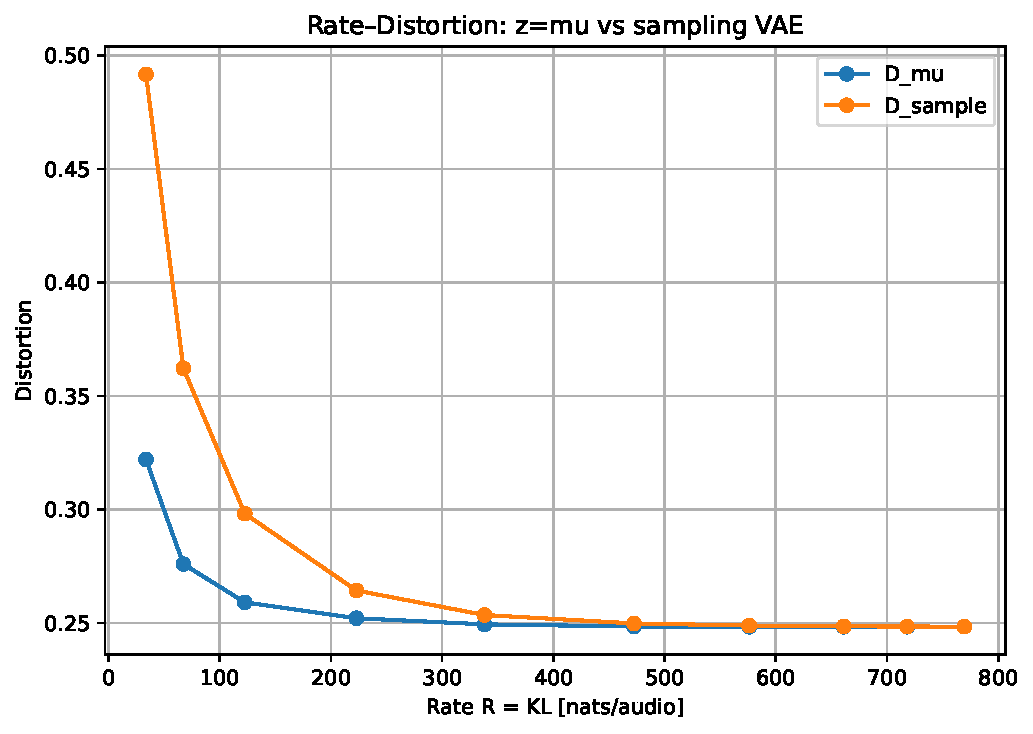
\includegraphics[width=0.98\linewidth]{figures/rate_distortion.pdf}
    \caption{Rate--distortion curve. At low Rate, distortion under sampling increases much more rapidly than distortion evaluated using $z=\mu$.}
    \label{fig:rd}
\end{figure}


% ------------------------------------------------------------------------------
\section*{What changes in the latent space?}

All 128 latent dimensions remain active using the threshold $\mathrm{KL}_i>0.01$, while the effective dimensionality decreases only moderately, from about 123 to 115. Thus, the Rate reduction is not mainly due to coordinate shutdown: instead, $|\mu|$ decreases and the mean posterior standard deviation moves toward 1. Across the four main regimes, $\bar{\sigma}$ increases from 0.229 to 0.771, while $G_{\mathrm{stoch}}$ rises from 0.0041 to 0.1697.

% ------------------------------------------------------------------------------
\section*{Controlled perturbation of the latent space}

To isolate latent stochasticity, we keep the model fixed and define
\begin{equation}
z_\tau = \mu + \tau\sigma\odot\epsilon,
\qquad
\epsilon\sim\mathcal{N}(0,I).
\end{equation}

In latent space,
\begin{equation}
\mathbb{E}\|z_\tau-\mu\|^2
=
\tau^2\sum_i\sigma_i^2,
\end{equation}

which is matched by Monte Carlo estimates with relative discrepancy below $0.6\%$. A local decoder linearization,
\begin{equation}
g_\theta(z_\tau)
\approx
g_\theta(\mu)+
\tau J_{g_\theta}(\mu)\mathrm{diag}(\sigma)\epsilon,
\end{equation}

implies
\begin{equation}
\mathbb{E}\|g_\theta(z_\tau)-g_\theta(\mu)\|^2
\approx c\tau^2.
\end{equation}

For $\tau\leq1$, all fits achieve $R^2>0.998$. The coefficient $c$ increases from $0.0045$ to $0.1843$ as the Rate decreases from about $338$ to $34$ nats/audio (Figure~\ref{fig:sens}).

\begin{figure}[t]
    \centering
    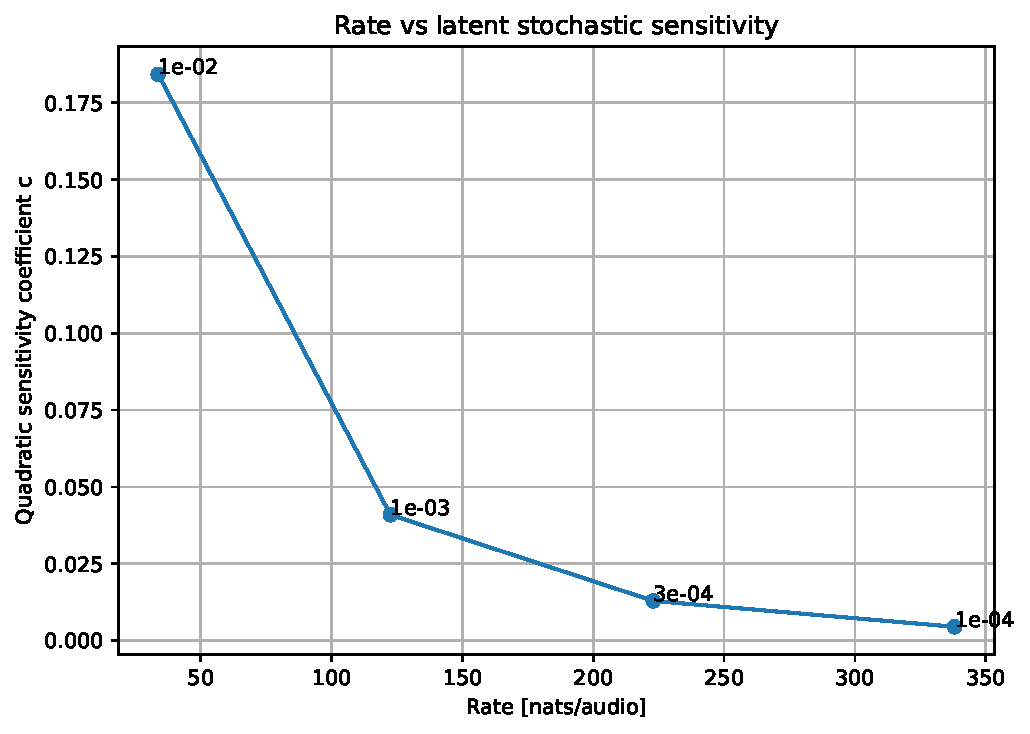
\includegraphics[width=0.98\linewidth]{figures/rate_sensitivity.pdf}
    \caption{The quadratic coefficient $c$ increases as the Rate decreases: more compressed models are more sensitive to latent stochastic perturbations.}
    \label{fig:sens}
\end{figure}

% ------------------------------------------------------------------------------
\section*{Robustness and conclusions}

Repeating VAE fine-tuning with three random seeds, always starting from the same pre-trained autoencoder, gives the results reported in Table~1.

\begin{table}[t]
\centering
\caption{Mean $\pm$ standard deviation over three random seeds.}
\label{tab:seed}
\begin{tabular}{cccc}
\toprule
$\beta$ & $R$ & $\bar{\sigma}$ & $G_{\mathrm{stoch}}$ \\
\midrule
$10^{-4}$ & $339.4\pm1.3$ & $0.226\pm0.002$ & $0.0039\pm0.0004$ \\
$10^{-3}$ & $119.5\pm2.6$ & $0.475\pm0.009$ & $0.0400\pm0.0004$ \\
$10^{-2}$ & $32.4\pm1.6$ & $0.792\pm0.022$ & $0.1672\pm0.0047$ \\
\bottomrule
\end{tabular}
\end{table}

The trends remain stable across seeds. Decreasing the Rate pushes the posterior toward the prior ($\mu\rightarrow0$, $\sigma\rightarrow1$) and increases the cost of latent sampling. Therefore, evaluating the VAE only through $z=\mu$ can underestimate reconstruction distortion in low-Rate regimes. The association between $\bar{\sigma}$ and $G_{\mathrm{stoch}}$ is consistent with the reparameterization mechanism, but should not be interpreted as isolated causal evidence. The multi-seed analysis is limited to VAE fine-tuning from the same pre-trained autoencoder.

\section*{Quantitative interpretation of the trade-off}

To compare regimes with different baseline distortions, we define the relative stochasticity gap

\begin{equation}
G_{\mathrm{rel}}
=
100\frac{D_{\mathrm{sample}}-D_\mu}{D_\mu}.
\end{equation}

It increases from $1.6\%$ at $\beta=10^{-4}$ to $4.8\%$ at $3\cdot10^{-4}$, $15.1\%$ at $10^{-3}$, and $52.7\%$ at $10^{-2}$, showing that posterior-mean reconstruction becomes increasingly optimistic at low Rate.

The local approximation also gives

\begin{equation}
c \approx
\mathbb{E}_x
\left[
\left\|
J_{g_\theta}(\mu)\,
\mathrm{diag}(\sigma)
\right\|_F^2
\right],
\end{equation}

so $c$ reflects both posterior uncertainty and local decoder sensitivity. The clearest transition occurs between $R\simeq223$ and $122$ nats/audio. Independent audio metrics show the same behavior, supporting the conclusion that the effect is not specific to the weighted log-STFT loss.

\clearpage

% ------------------------------------------------------------------------------
\section*{Statement on the use of AI}

The general topic of the project was identified independently by the author. ChatGPT (OpenAI) was then used as a guide to refine this initial idea into a more specific research question and to support part of the writing and debugging of the Python code. All numerical experiments were executed locally by the author, and the resulting outputs were checked throughout the development of the project. Final responsibility for the content, verification of the results, and understanding of all submitted material remains with the author.

\bibliography{references.bib}
\bibliographystyle{dlaiml2026}

\clearpage
\section*{Appendix}

\paragraph*{A. Effective latent dimensionality.}
The effective latent dimensionality remains high along most of the rate--distortion curve and decreases visibly only in the very low-Rate regimes.

\begin{minipage}{\linewidth}
\centering
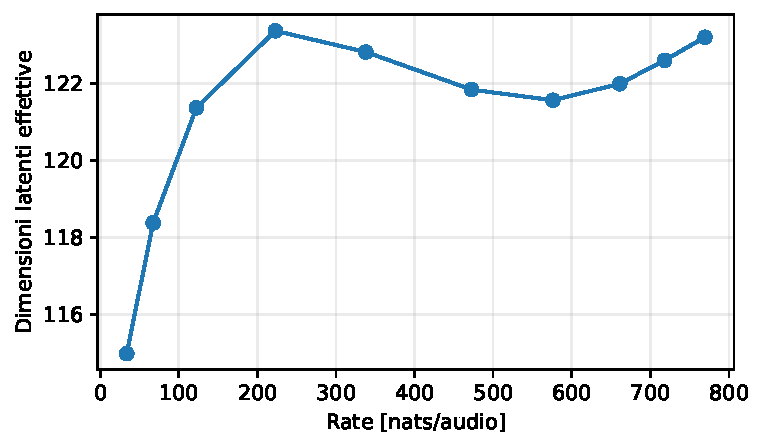
\includegraphics[width=0.90\linewidth]{figures/rate_effective_dims.pdf}

\emph{Figure A1.} Rate vs effective latent dimensionality.
\end{minipage}

\paragraph*{B. Posterior uncertainty.}
The mean posterior standard deviation increases as the Rate decreases, consistently with $q_\phi(z|x)$ approaching the standard normal prior.

\begin{minipage}{\linewidth}
\centering
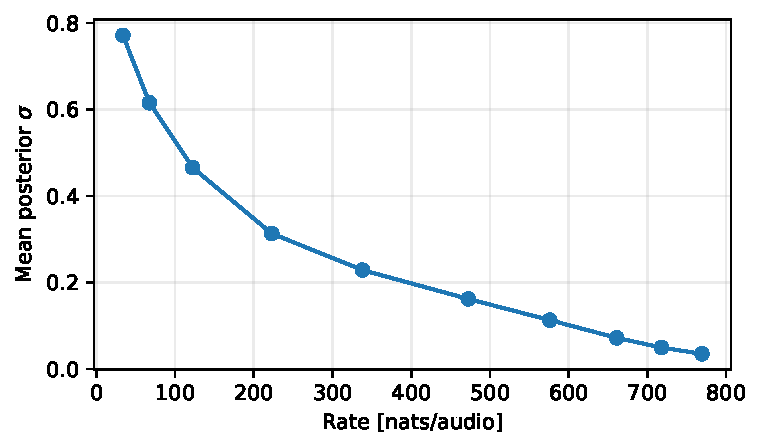
\includegraphics[width=0.90\linewidth]{figures/rate_sigma.pdf}

\emph{Figure A2.} Rate vs mean posterior standard deviation.
\end{minipage}

\paragraph*{C. Controlled perturbations in $\tau$.}
The output displacement grows approximately linearly with $\tau^2$ for $\tau\leq1$; for larger perturbations, nonlinear decoder effects become increasingly visible.

\begin{minipage}{\linewidth}
\centering
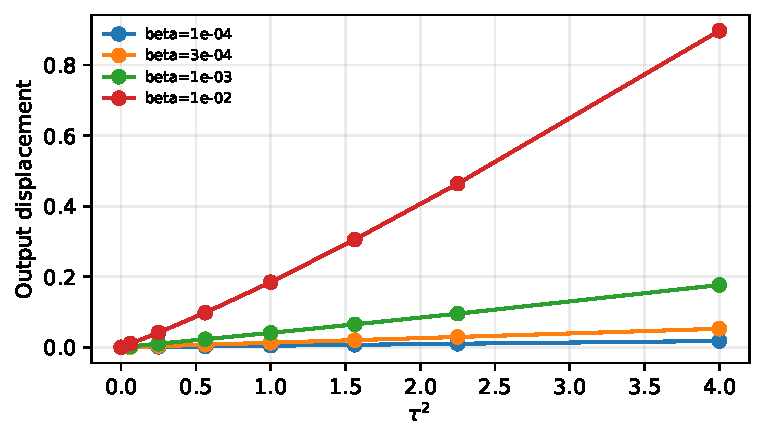
\includegraphics[width=0.90\linewidth]{figures/tau_output_displacement.pdf}

\emph{Figure A3.} Output displacement as a function of $\tau^2$.
\end{minipage}

Reconstruction distortion increases with $\tau$, particularly for low-Rate models.

\begin{minipage}{\linewidth}
\centering
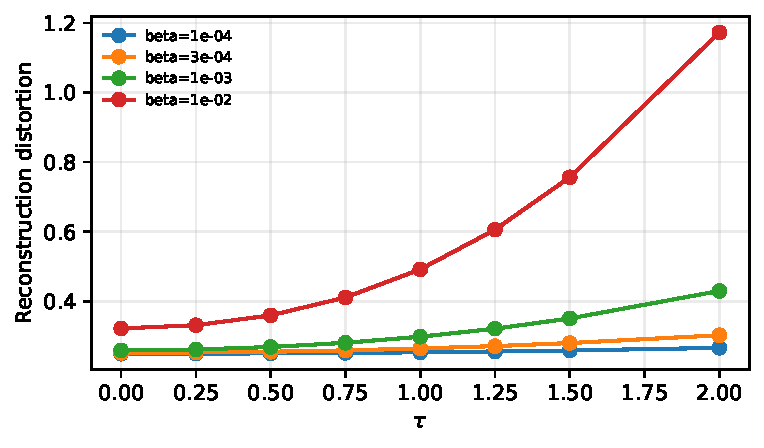
\includegraphics[width=0.90\linewidth]{figures/tau_reconstruction.pdf}

\emph{Figure A4.} Reconstruction distortion as a function of $\tau$.
\end{minipage}

\paragraph*{D. Robustness across random seeds.}
The mean stochasticity gap increases as the Rate decreases, and the association between posterior uncertainty and the stochasticity gap remains stable across the three fine-tuning seeds.

\begin{minipage}{\linewidth}
\centering
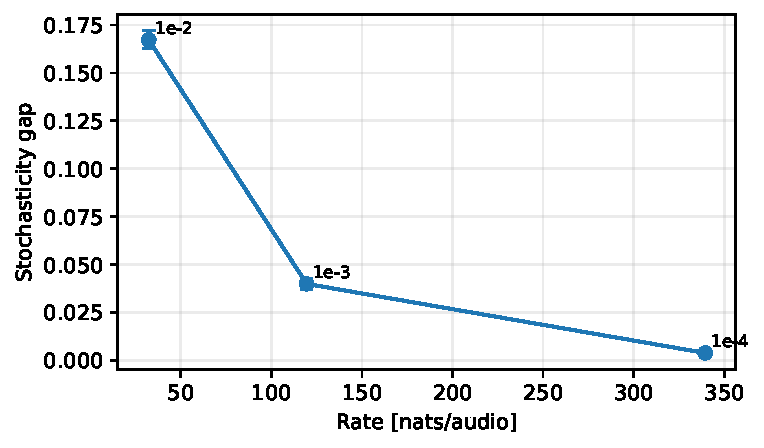
\includegraphics[width=0.90\linewidth]{figures/seed_gap_rate.pdf}

\emph{Figure A5.} Mean stochasticity gap across seeds as a function of Rate.
\end{minipage}

\begin{minipage}{\linewidth}
\centering
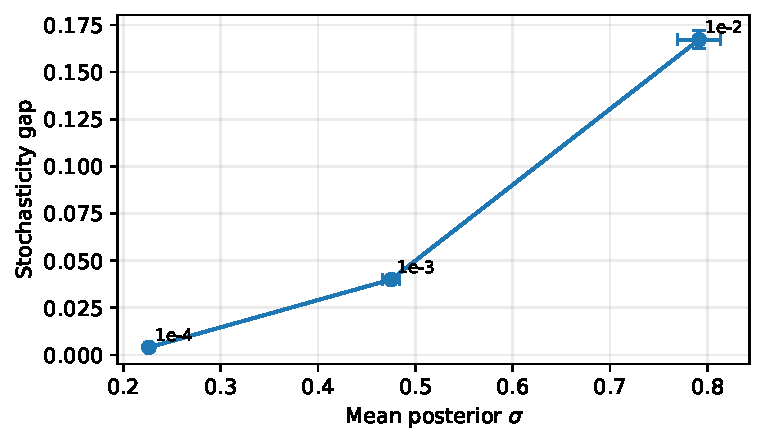
\includegraphics[width=0.90\linewidth]{figures/seed_sigma_gap.pdf}

\emph{Figure A6.} Posterior uncertainty vs stochasticity gap with error bars.
\end{minipage}

\paragraph*{E. Audio metrics.}
On the active speech region, the metrics obtained under posterior sampling are:

\begin{minipage}{\linewidth}
\centering
\begin{small}
\begin{tabular}{cccc}
\toprule
$\beta$ & MSE & SNR & LogMelMAE\\
\midrule
$10^{-4}$ & 0.000478 & 5.671 & 7.189\\
$3\cdot10^{-4}$ & 0.000510 & 5.483 & 7.274\\
$10^{-3}$ & 0.000581 & 5.002 & 7.641\\
$10^{-2}$ & 0.000958 & 2.943 & 9.345\\
\bottomrule
\end{tabular}
\end{small}
\end{minipage}

\end{document}
